\chapter{Mathematical background}
\label{chpr:math}
The present study starts with an introduction to the mathematical foundations required for its understanding. The reader that is familiar with abstract algebra and elliptic curve cryptography may skip the first chapter to deal directly with the digital signature schemes presented in Chapter \ref{chpr:dss}.
\\
We start with a brief presentation of the group and field's structures, deferring the introduction to elliptic curves mathematics to the second section.

\bigskip

\section{Groups and fields}
\label{chpr:groupsfields}

\begin{mydef} {\bf (Group)}: A group is a non empty set $G$ together with a binary operation $\bullet$ (called the 	group law of $G$) that satisfies:
	\begin{itemize}
		\item Closure: $\forall a, b \in G  \Longrightarrow a \bullet b \in G$;
		\item Associativity: $\forall a, b, c \in G  \Longrightarrow (a \bullet b) \bullet c = a \bullet (b \bullet c)$;
		\item Identity: $\exists e \in G \ | \ \forall a \in G, \ e \bullet a = a \bullet e = a$. Such an element $e$ is unique; 
		\item Invertibility: $\forall a \in G, \ \exists b \in G \ | \ a \bullet b = b \bullet a = e$. This element is unique and it is commonly denoted either as $a^{-1}$ or $-a$, depending on the notation (multiplicative or additive).
	\end{itemize}
\end{mydef}
\label{def1}
As a careful reader may have noticed, it is not required the property of commutativity. This means that, in general, the result of the operation may depend on the order of the operands. If this is not the case, meaning that the group operation is also commutative, the group is called abelian.
\\
Consider now a group $(G, +)$: hereinafter we will stick with the additive notation.
If $G$ is finite, i.e. it has a finite number of elements, we define the order of $G$ as the number of elements in $G$. We can also define the order of an element $g \in G$ to be the smallest integer $k > 0$ such that $kg = 0$\footnote{In an additive group it is natural to define the scalar multiplication: given $g \in G$ and $k \in \mathbb{N}, \ k \neq 0$, we have that $kg = g + g + ... + g$, where the summation is repeated $k - 1$ times. In a similar fashion, it is natural to define exponentiation in the multiplicative case.}, where with 0 we denote the additive identity. If $k$ is the order of $g$, then:
$$ig = jg \Longleftrightarrow i \equiv j \ (\text{mod} \ k).$$
Indeed:
$$ig = jg \ \Longleftrightarrow \ (i - j)g = 0 \ \Longleftrightarrow \ i - j = nk, \ n \in \mathbb{Z}\text{\textbackslash}\{0\},$$
from which the thesis.
\\
Next we state one basic result in group theory, that will turn out to be very useful in the following:
\begin{thm} {\bf (Lagrange's theorem)}:
	Let $G$ be a finite group.
	\begin{enumerate}
		\item Let $H$ be a subgroup\footnote{Given a group $(G, +)$, a subset $H$ is a subgroup of $G$ if $H$ endowed with the restriction of the group operation to $H \times H$ is a group.} of $G$. Then the order of $H$ divides the order of $G$;
		\item Let $g \in G$. Then the order of $g$ divides the order of $G$.
	\end{enumerate}
\end{thm}

\bigskip

\noindent
For the cryptographic applications that we will study a particular family of groups turn out to be very important: cyclic groups. A cyclic group is a group that is generated by a single element: this means that it contains (at least) an element $g$ such that every other element of the group can be obtained by repeatedly applying the group operation to $g$, i.e. $\forall h \in G, \ \exists n \in \{1, ..., k\} \ | \ h = ng$, where $k$ as before denotes the order of $g$. All the group's elements satisfying this property are called generator of the group.
\\
Two interesting properties of cyclic groups are the following:
\begin{enumerate}
	\item Every cyclic group is abelian;
	\item Every finite group has at least a cyclic subgroup.
\end{enumerate}

\bigskip
\noindent
Now let's get to the mathematical concept of field. A field is a non empty set on which are defined two binary operations, usually called addition and multiplication. It has to be an abelian group under addition (with 0 denoting the additive identity) and the non-zero elements have to form an abelian group under multiplication. Finally, the multiplication has to be distributive over addition. 
\\
More precisely we can give the following definition.
\begin{mydef} {\bf (Field)}: A field is a set $K \neq \emptyset$ endowed with two binary operations $+$ and $*$, such that:
\begin{itemize}
	\item $(K, +)$ is an abelian group, whose identity element is denoted by 0. This group is called the additive group of the field;
	\item $(K \text{\textbackslash}\{0\}, *)$ is an abelian group. This is called the multiplicative group of the field, sometimes denoted by $K^{\times}$ or by $K^*$;
	\item $\forall a \in K \text{\textbackslash} \{0\}, \ \forall b, c: \ a * (b + c) = a * b + a * c$. 
\end{itemize}
\end{mydef}

\bigskip
\noindent
Another key role in the following will be played by finite fields: a finite field is simply a field with a finite number of elements. It can be shown that a finite field of order $q$, denoted as $\mathbb{F}_q$, exists if and only if $q = p^k$, where $p$ is a prime number and $k$ is a positive integer. The field of a given order is unique, up to an isomorphism (this means that there are different representations of a unique mathematical object). In a field of order $p^k$, the characteristic of the field (as defined below) is $p$: thus adding $p$ copies of any element results in the additive identity. 
\\
In particular we will deal with prime finite fields, i.e. the finite fields whose order is a prime number. Finite fields of order a prime $p$ may be represented by the set $\{0, 1, ..., p-1\}$ with addition and multiplication defined through modular arithmetic, that is: given $a, b \in \mathbb{F}_p$ then $r = a + b$ and $s = a * b$ are integers in $[0, p - 1]$, defined as the remainder of the divisions $(a + b)/p$ and $a*b/p$, respectively. This is usually written as: $a + b \equiv r \ (\text{mod} \ p)$ and $a * b \equiv s \ (\text{mod} \ p)$ or as $a + b \equiv r \ \text{in} \ \mathbb{F}_p$ and $a * b \equiv s \ \text{in} \ \mathbb{F}_p$ . It is easy to see that in this case the additive identity is the integer 0, while the multiplicative identity is the integer 1.
\\
Subtraction and division are defined via the additive and multiplicative inverses:
\begin{itemize}
	\item Subtraction: given $a \in \mathbb{F}_p$, we know by definition that there is a unique element $-a \in \mathbb{F}_p$ such that $a + (-a) = 0 \ (\text{mod} \ p)$. Then we define subtraction as: $a - b = a + (-b) \ (\text{mod} \ p), \ \forall a, b \in \mathbb{F}_p$;
	\item Division: $\forall a \in \mathbb{F}_p \text{\textbackslash} \{0\}, \ \exists a^{-1} \ | \ a * a^{-1} = 1 \ (\text{mod} \ p)$, again by the definition. Thus we can defined division as: $a / b = a * (b)^{-1}, \ \forall a, b \in \mathbb{F}_p \text{\textbackslash} \{0\}$.
\end{itemize}
Notice that not all the finite fields $\mathbb{F}_q$ are isomorphic to $\mathbb{Z}_q$: consider for example the case $q = 2^2 = 4$. Here $p = 2$ and $k = 2$. Since two is a prime number, we have that there exists a field with four elements. But since four is not a prime number, we cannot represent this field through the set $\mathbb{Z}_4 = \{0, 1, 2, 3\}$. Consider the element two: 2 * 0 = 0 (mod 4), 2 * 1 = 2 (mod 4), 2 * 2 = 0 (mod 4), 2 * 3 = 2 (mod 4). As we can see it does not admit a multiplicative inverse in $\mathbb{Z}_4$. 

\bigskip
\noindent
We end this section giving the definition of field characteristic, that will be useful when defining the equation of an elliptic curve. 
\begin{mydef} {\bf (Field characteristic)}: Given a field $(K, \ +, \ *)$, we denote by 0 and 1 the additive and multiplicative identities, respectively.
\\
The characteristic of $K$, denoted as  $\text{char}(K)$, is defined to be the smallest $n \in \mathbb{Z} \text{\textbackslash} \{0\}$ for which the following relation holds: 
$$\underbrace{1 + ... + 1}_\text{$n$ times} = 0$$ 
In case this relation never holds, the field is said to have characteristic zero.
\end{mydef}

\bigskip

\bigskip

\section{Introduction to elliptic curves}
\label{chpr:ec}
An elliptic curve over a field $K$ is a non-singular cubic curve in two variables: it is defined by the equation $f(x, y) = 0$, where $f$ is a polynomial in $x$ and $y$ of degree three with coefficients in $K$.
\\
In the most general case, an elliptic curve is defined through the following equation: $y^2 + a_1xy + a_2y = x^3 + a_3x^2 + a_4x + a_5$, where $a_1, ..., a_5 \in K$. This form is called generalized Weierstrass equation, and can be simplified according to the characteristic of the field. In particular, if it is different from two and three we can write:
$$y^2 = x^3 + ax + b, \ a, b \in K.$$
This latter equation is called Weierstrass equation, and it is the most widely used.
\\
We will denote an elliptic curve over a field $K$ through the notation $E(K)$, that represents the set of points satisfying the defining equation. By construction, this set also contains a special point, called the point at infinity (its role will be clarified in the next section): 
$$E(K) = \{\infty\}\cup\{(x, y) \in K \times K \ | \ y^2 = x^3 + ax + b\}.$$
\\
To start familiarizing with elliptic curves, it could be useful to consider the case in which $K = \mathbb{R}$, the set of real numbers. In Figure \ref{fig:figure1} we can look at a couple of elliptic curves' real graph.
\begin{figure}
	\noindent
	\makebox[\textwidth]{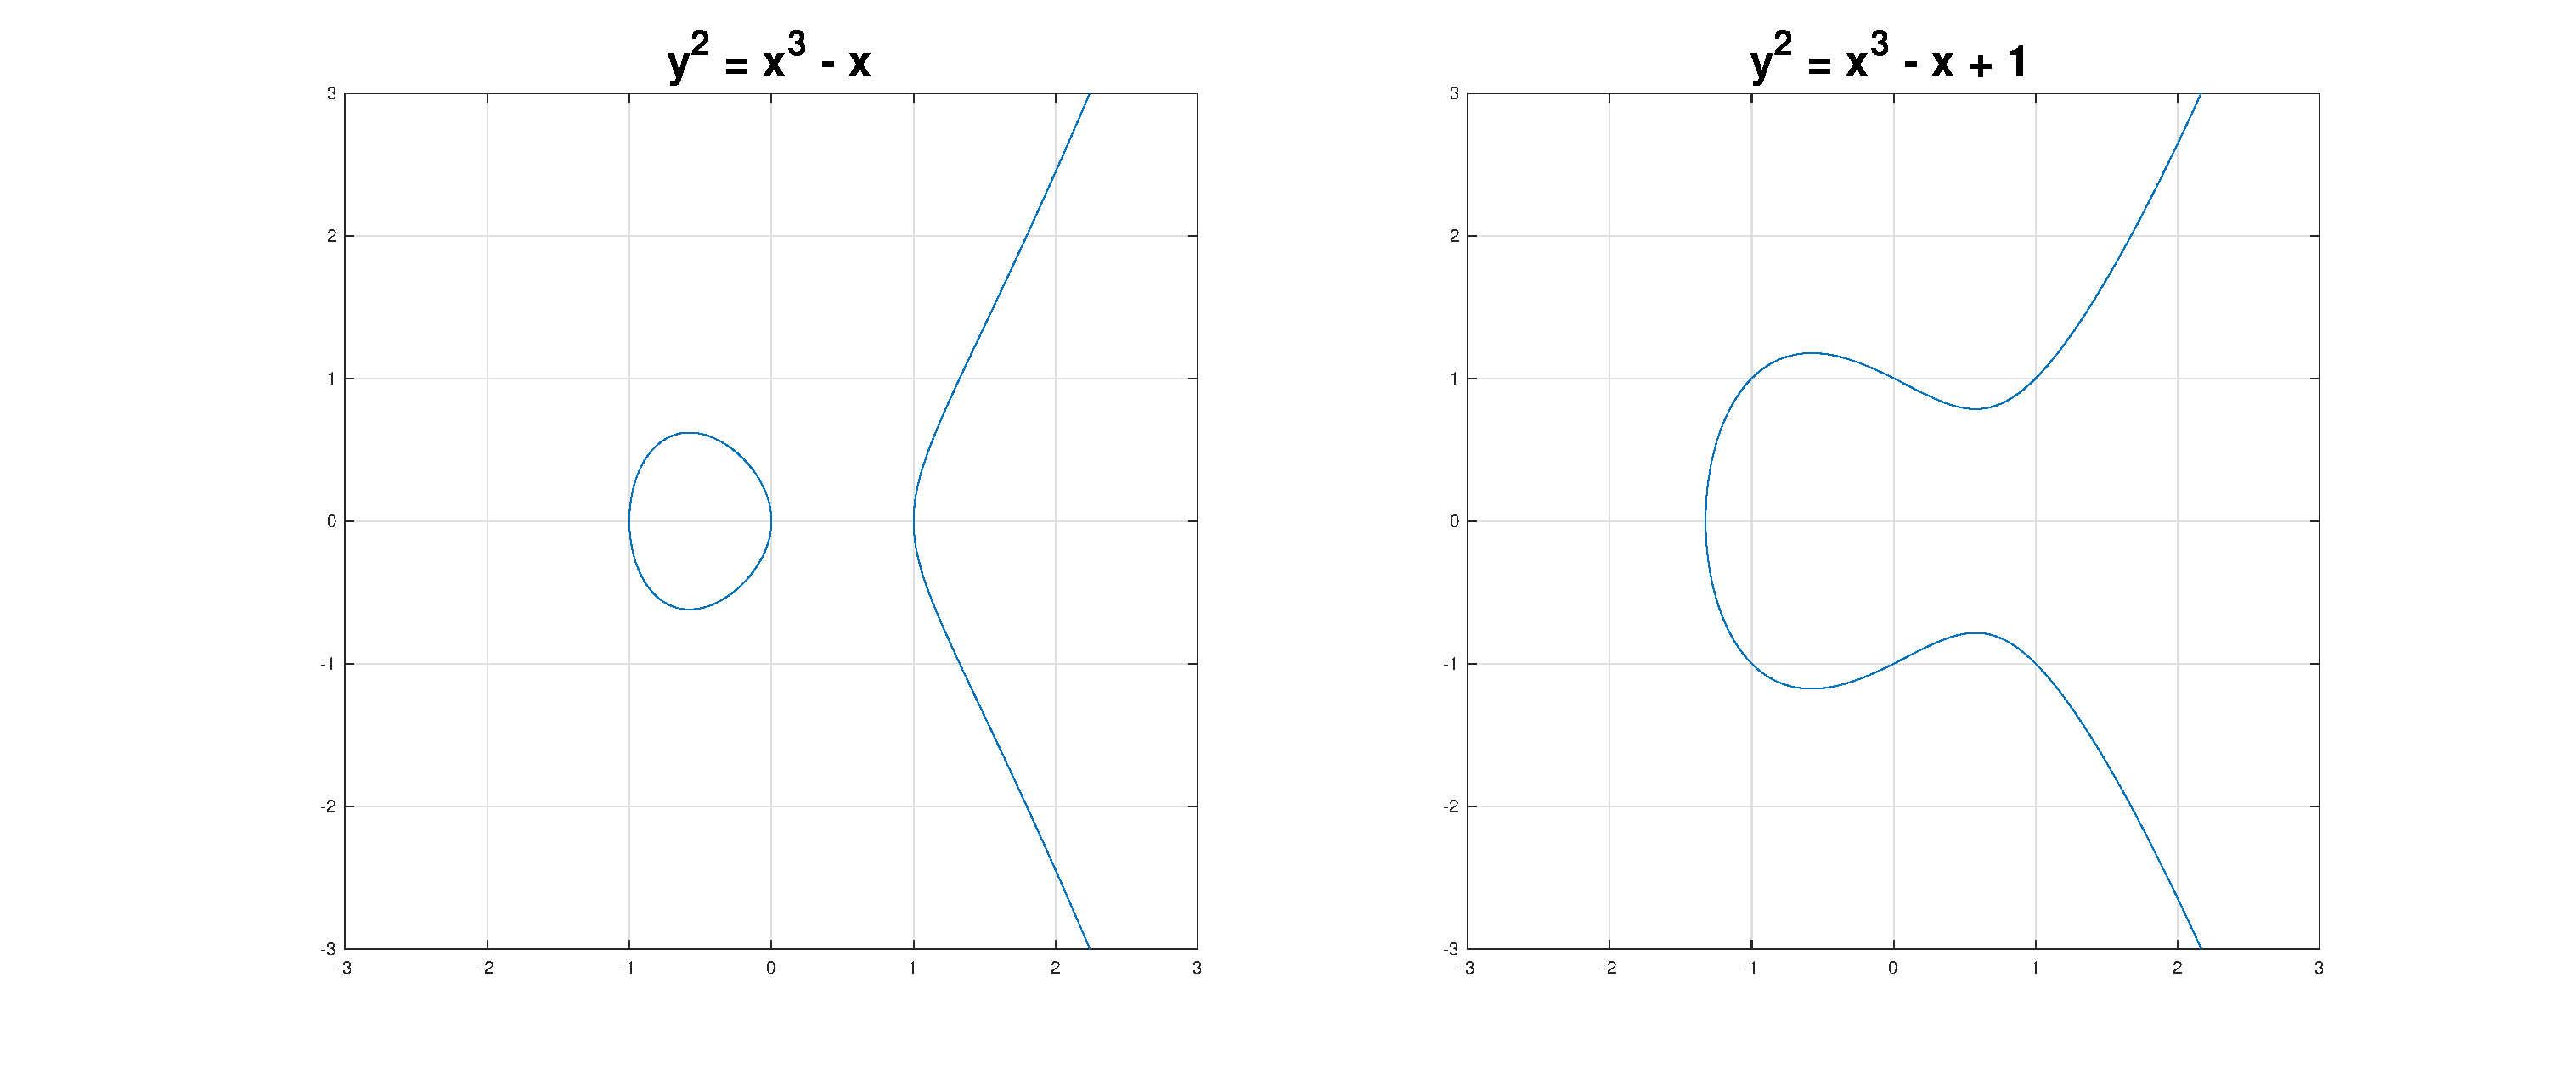
\includegraphics[width=15cm, height=7cm]{Images/EC.eps}}
	\captionof{figure}{Two examples of elliptic curves over the real numbers.}
	\label{fig:figure1}
\end{figure}
\noindent
As we can see, the elliptic curves are symmetric with respect to the $x$-axis, so that for every feasible $x$ there are two $y$ values satisfying the Weierstrass equation.
\\
Typically the Weierstrass equation is coupled with the constraint that the discriminant of the cubic $x^3 + ax + b$ is different from zero. This is equivalent to ask that:
$$4a^3 + 27b^2 \neq 0,$$ 
in order to avoid multiple roots. Geometrically, this requirement means that there are no cusps, self intersections or isolated points\footnote{This requirement has also other implications: it can be shown that, without it, the elliptic curve $E_{ns}(K)$ defined over the non-singular points has an isomorphism with simpler algebraic structures, such as $K$ itself or $K^{\times}$. This problem typically arises when dealing with elliptic curves modulo composites.}. 
We can also link the sign of the discriminant to the number of components of the curve: the real graph of a curve has two components if its discriminant is positive, and one component if it is negative, as exemplified in Figure \ref{fig:figure1}.

\bigskip
\noindent
We get back for a moment to the generalized Weierstrass equation, and show how to go from there to the more appealing Weierstrass form:
$$y^2 + a_1xy + a_2y = x^3 + a_3x^2 + a_4x + a_5,$$ 
with $a_1,...,a_5$ constants in $K$. We have said that this is the most generic form for an elliptic curve, but what does it exactly mean? It means that it is always possible to reduce to the Weierstrass equation, unless the characteristic of the field over which the curve is defined is two or three. In these two cases, we need to resort to the general formula.
\\
However, if the characteristic of the field is not two we can divide by two\footnote{Remember that in a field of characteristic two the number two acts as zero, the additive element that has not a multiplicative inverse.} and complete the square: $$\left(y + \frac{a_1x}{2} + \frac{a_2}{2}\right)^2 = x^3 + \left(a_3 + \frac{a_1^2}{4}\right)x^2 + \left(a_4 + \frac{a_1a_2}{4}\right)x + \left(\frac{a_2^2}{4} + a_5\right),$$ which can be written as $$y_1^2 = x^3 + a_1{'}x^2 + a_2{'}x + a_3{'},$$ with $y_1 = y + \frac{a_1x}{2} + \frac{a_2}{2}$ and new constants $a_1{'}, a_2{'}, a_3{'}$. Moreover, if the characteristic is neither three, then we can consider $x_1 = x + \frac{a_1{'}}{3}$:
$$y_1^2 = x^3 + a_1{'}x^2 + a_2{'}x + a_3{'} = \left(x_1 - \frac{a_1{'}}{3}\right)^3 + a_1{'}\left(x_1 - \frac{a_1{'}}{3}\right)^2 + a_2{'}\left(x_1 - \frac{a_1{'}}{3}\right) + a_3{'} = $$ $$= \left(x_1 - \frac{a_1{'}}{3}\right)\left(x_1^2 + \frac{a_1{'}^2}{9} -\frac{2}{3}a_1{'}x_1 + a_1{'}x_1 - \frac{a_1{'}^2}{3} + a_2{'}\right) + a_3{'} = $$ $$=\left(x_1 - \frac{a_1{'}}{3}\right) \left(x_1^2 + \frac{1}{3}a_1{'}x_1 - 	\frac{2}{9}a_1{'}^2 + a_2{'}\right) + a_3{'} = $$ $$= x_1^3 + \cancel{\frac{1}{3}a_1{'}x_1^2} - \frac{2}{9}a_1{'}^2x_1 + a_2{'}x_1 - \cancel{\frac{1}{3}a_1{'}x_1^2} - \frac{1}{9}a_1{'}^2x_1 + \frac{2}{27}a_1{'}^3 - \frac{1}{3}a_1{'}a_2{'} + a_3{'} = $$ $$=x_1^3 + \left(a_2{'} - \frac{1}{3}a_1{'}^2\right)x_1 + \left(\frac{2}{27}a_1{'}^3 - \frac{1}{3}a_1{'}a_2{'} + a_3{'}\right).$$ 
Through a proper renaming of the constants we get finally to the well known Weierstrass form: $y_1^2 = x_1^3 + ax_1 + b$ for some constants $a$ and $b$ in $K$. 
\\
Finally we present the case of the equation $cy^2 = dx^3 + ax + b$ and how to transform it in Weierstrass form. We can multiply both sides by $c^3d^2$ and write $(c^2dy)^2 = (cdx)^3 + (ac^2d)(cdx) + bc^3d^2$. The change of variables $y_1 = c^2dy$ and $x_1 = cdx$ yields to the desired formulation of the equation.

\bigskip

\bigskip

\section{The group law}
\label{chpr:grouplaw}
This section is devoted to the definition of an addition operation between elements in $E(K)$: this operation turns out to be fundamental since it induces the structure of abelian group on the elliptic curve's point. Moreover, we will see why, in the definition of the curve, we had to consider the point at infinity.
\\
In particular we will consider $K$ to be the set of real numbers, in order to give an easy graphical representation of the operation. This can be done without loss of generality, since the formulas that we will derive can be shown to be valid for every $K$ with $\text{char}(K) \neq 2, 3$. 

\bigskip
\noindent
Loosely speaking we can say that:
\begin{itemize}
	\item The points of the elliptic curve are the group's elements;
	\item The identity element is the point at infinity, denoted by $\infty$;
	\item The inverse of a point $Q$ is the one symmetric about the $x$-axis: $Q = (x, y) \Longrightarrow -Q = (x, -y)$;
	\item Addition is given by the following rule: given three aligned points on the curve $Q_1$, $Q_2$ and $Q_3$ their sum is $Q_1 + Q_2 + Q_3 = \infty$.  
\end{itemize}

\begin{center}
	\noindent
	\makebox[\textwidth]{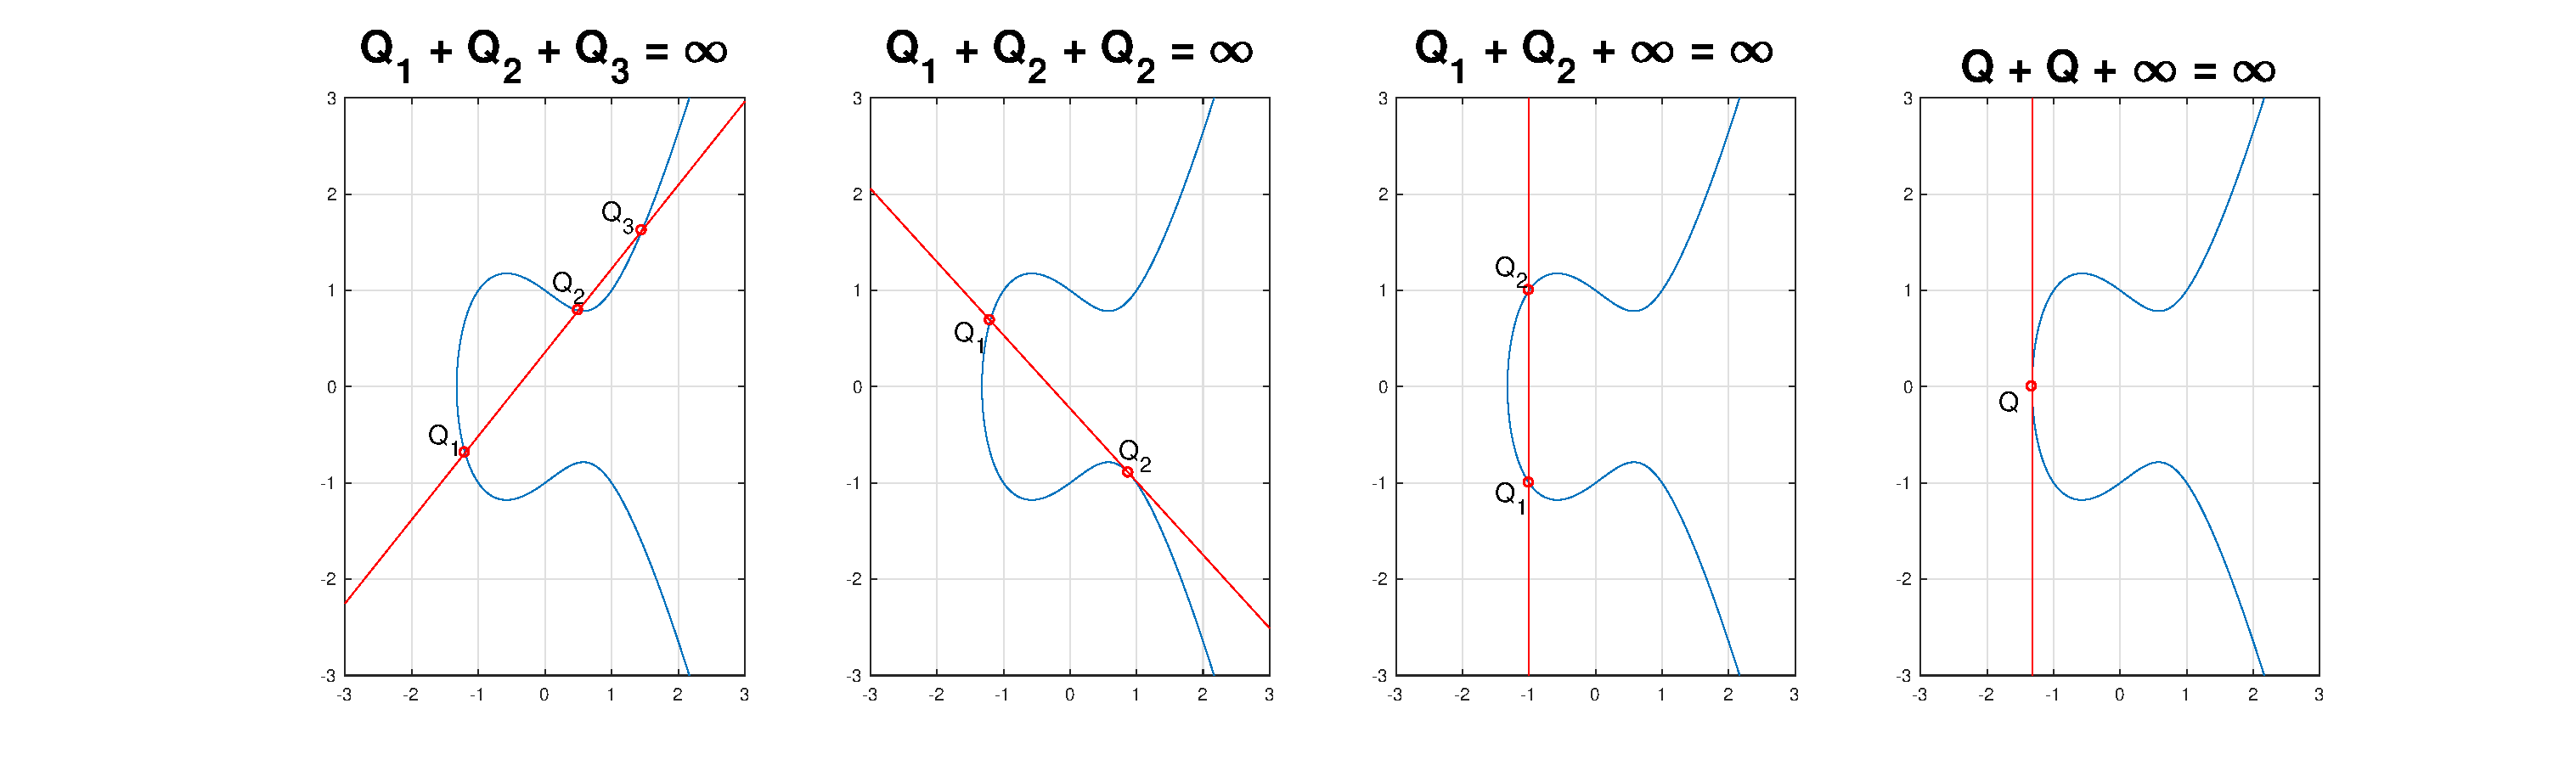
\includegraphics[width=20cm, height=5cm]{Images/chord.eps}}
	\captionof{figure}{Geometrical interpretation of the addition of EC points.}
	\label{fig:figure2}
\end{center}
\noindent
In order to define properly the addition of EC points we need to consider five different cases. We start taking an elliptic curve $E$ defined by the usual equation in Weierstrass form $y^2 = x^3 + ax + b, \ a,b \in \mathbb{R}$ and two points $Q_1 = (x_1, y_1), Q_2 = (x_2, y_2) \in E$. Unless otherwise specified, we assume also that $Q_1, Q_2 \neq \infty$.
\begin{enumerate}
	\item $x_1 \neq x_2$: consider the line passing through $Q_1$ and $Q_2$. In most of the cases (i.e. when neither the points are tangent points) this line will intersect the curve in a third point, that we denote as $-Q_3$. Then take the reflection with respect to the $x$-axis (i.e. change the sign of the $y$ coordinate): denote this final point as $Q_3$.
	\\
	The algorithm specified allows us to give meaning to the formula: 
	$$Q_1 + Q_2 = Q_3.$$
	The one outlined above is the geometrical intuition, but we can obtain algebraic formulas for the operation. The line passing through $Q_1$ and $Q_2$ has equation $y = m(x - x_1) + y_1$, where $m = \frac{y_2 - y_1}{x_2 - x_1}$ is its slope. Notice that if $x_1 = x_2$ the line is vertical, but we will treat this case later on. We can find the intersections between the line and the curve through a substitution: $(m(x - x_1) + y_1)^2 = x^3 + ax + b$. We have $m^2(x^2 - 2x_1x + x_1^2) + 2my_1(x - x_1) + y_1^2 = x^3 + ax + b$; this formula can be rearranged in the form: $$x^3 - m^2x^2 + (a + 2m^2x_1 - 2my_1)x + (b + 2my_1x_1 - m^2x_1^2 -y_1^2) = 0.$$
	\\
	In general solving a cubic equation is non trivial, but we have already two roots, namely $x_1$ and $x_2$ since $Q_1$ and $Q_2$ are points on both the line and the curve. To find the third root we notice that, given a cubic polynomial $x^3 + ax^2 + bx + c$ with roots $r, s$ and $t$, we can write: $$x^3 + ax^2 + bx + c = (x - r)(x - s)(x - t) =$$ 
	$$= x^3 - (r + s + t)x^2 + (rs + rt + st)x - rst.$$
	Therefore $r + s + t = - a$, so that, if we know two roots $r$ and $s$, we can find the third as $t = - a - r - s$.
	\\
	In our case we have $x_1 + x_2 + x_3 = m^2 \ \Longrightarrow \ x_3 = m^2 - x_1 - x_2$. Remembering to change the $y$ coordinate of the intersection point due to the reflection, we get $Q_3$ as: $x_3 = m^2 - x_1 - x_2$ and $y_3 = m(x_1 - x_3) - y_1$.
	\begin{figure}
		\noindent
		\makebox[\textwidth]{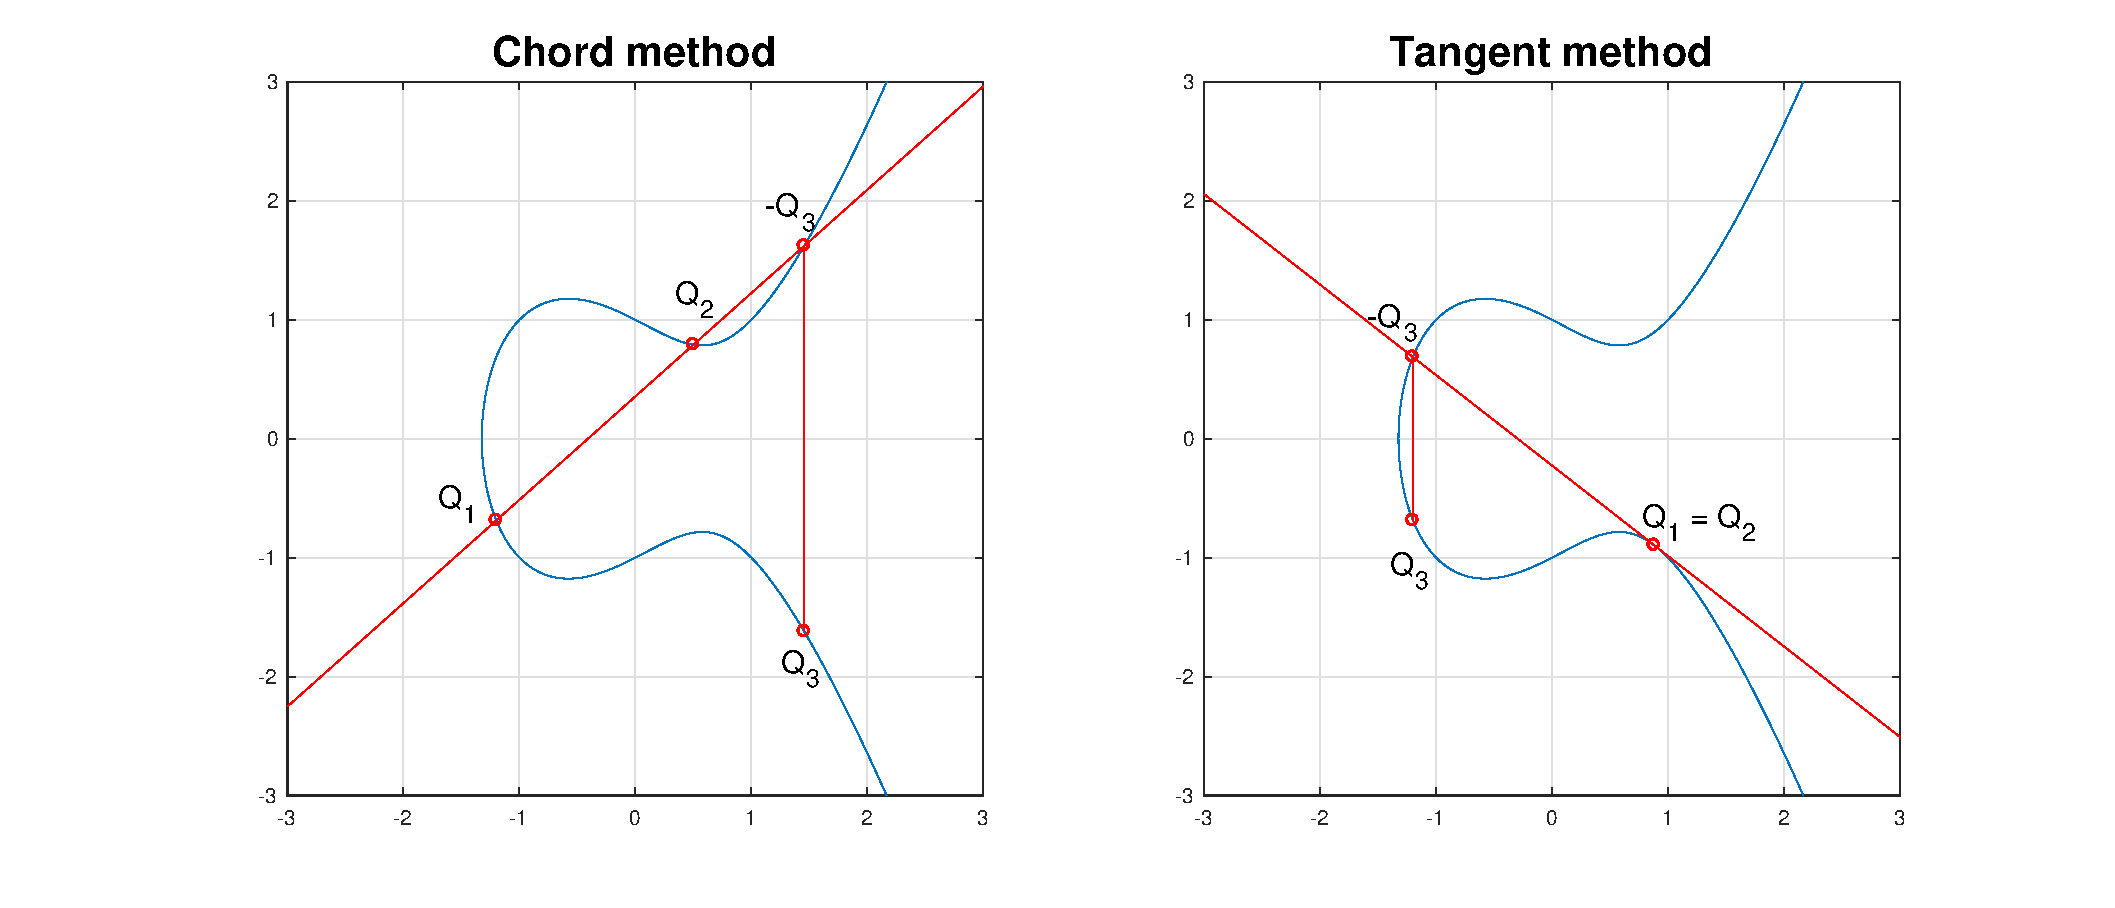
\includegraphics[width=15cm, height=7cm]{Images/sum.eps}}
		\captionof{figure}{Point addition: graphical representation.}
		\label{fig:figure3}
	\end{figure}
	
	\item $x_1 = x_2 \wedge y_1 \neq y_2$: the line through $Q_1$ and $Q_2$ is vertical, therefore it intersects $E$ at $\infty$. Reflecting the point at infinity across the $x$-axis yields to the same point. Therefore, in this case $Q_1 + Q_2 = \infty$. 
	\\
	This is in agreement with what we stated before: if  $x_1 = x_2 \wedge y_1 \neq y_2$ it means that $Q_2 = -Q_1$, and since the point at infinity acts as the identity element we have exactly that $Q_1 + Q_2 = \infty$.
	
	\item $Q_1 = Q_2 = (x_1, y_1) \wedge y_1 \neq 0$: when two points on a curve are very close one another, the line through them approximates a tangent line. Therefore, when the two points coincide, we take the line through them to be the tangent line. Implicit differentiation allows us to find its slope $m$:
	$$y^2 = x^3 + ax + b \ \Longrightarrow \ \frac{d(y(x)^2)}{dx} = \frac{d}{dx}(x^3 + ax + b) \ \Longrightarrow$$
	$$ \Longrightarrow \ \frac{d(y^2)}{dy}\frac{dy}{dx}=2y\frac{dy}{dx}= 3x^2 + a \ \Longrightarrow $$ 
	$$\Longrightarrow \ m = \left(\frac{dy}{dx}\right)_{x_1} = \frac{3x_1^2 + a}{2y_1}.$$
	Again, the equation of the line is $y = m(x - x_1) + y_1$. At this point we can proceed as before: the line intersects the curve in a second point. Substituting the equation of the straight line would result in a cubic equation. But we already know two roots, so that we get: $x_3 = m^2 - 2x_1$ and $y_3 = m(x_1 - x_3) - y_1$.
	\\
	\item $Q_1 = Q_2 = (x_1, y_1) \wedge y_1 = 0$: as we can see from the previous point in this case the tangent line is vertical and we set $Q_1 + Q_2 = \infty$.
	\item The last case we have to deal with is when one of the two points is $\infty$. Suppose, without loss of generality, that $Q_2 = \infty$; the line through $Q_1$ and $\infty$ is a vertical line that intersects $E$ in the point $-Q_1$, which is the reflection of $Q_1$ across the $x$-axis. When we reflect $-Q_1$ to get $Q_3 = Q_1 + Q_2$, we get back to $Q_1$. Therefore:
	 $$Q_1 + \infty = Q_1$$
	for all points $Q_1$ on $E$. Of course, we extend this to include $\infty + \infty = \infty$.
\end{enumerate}
Thanks to these algebraic formulas we can notice that when $Q_1$ and $Q_2$ have coordinates in a field $K$ that contains $a$ and $b$, then $Q_1 + Q_2$ also has coordinates in $K$. This means that $E(K)$ is closed under the defined addition operation.

\bigskip
\noindent
Now we state a theorem showing formally that the couple $(E, +)$ is indeed an abelian group. The theorem with the proof can be found in \cite{RefWork:1}.
\begin{thm} The operation $+$ as defined above on an elliptic curve $E$ satisfies the following properties:
	\begin{enumerate}
		\item Commutativity: $Q_1 + Q_2 = Q_2 + Q_1, \ \forall Q_1, Q_2 \in E$;
		\item Identity: $Q + \infty = Q, \ \forall Q \in E$;
		\item Invertibility: $\forall Q \in E, \ \exists Q' \in E \ | \ Q + Q' = \infty$. This point will be denoted by $-Q$;
		\item Associativity: $(Q_1 + Q_2) + Q_3 = Q_1 + (Q_2 + Q_3), \ \forall Q_1, \ Q_2, Q_3 \in E$.
	\end{enumerate}
\end{thm}

\bigskip
\noindent
Although we won't prove the theorem, it can be useful to give a sketch of its proof. The commutativity is obvious, either from the formulas or from the fact that the line passing through $Q_1$ and $Q_2$ is the same as the line passing through $Q_2$ and $Q_1$. The identity property of the point at infinity holds by definition, as the existence of the inverse element.
\\
The tricky part of the proof is related with associativity: either it can be proved working out the annoying computations or through a much more elegant and complex method based on projective coordinates, for which we again refer to the bibliography.

\bigskip
\noindent
Now that we have clear in mind what does addition between EC points mean, we can define subtraction and scalar multiplication:
\begin{itemize}
	\item Subtraction: given $Q, R \in E$, we set $Q - R = Q + (-R)$. We can do this since everything is perfectly defined in the right hand side of the equation;
	\item Scalar multiplication: $\forall k \in \mathbb{N}$\textbackslash$\{0\}, \ kQ = Q + Q + ... + Q$, where the addition is repeated $k - 1$ times.
\end{itemize}
Notice that to compute the scalar multiplication for a large $k$ it is inefficient to add $Q$ to itself repeatedly. There are several faster approaches, the simplest called the {\bf double and add algorithm}. 
We stress this fact since, as we will see later on, scalar multiplication and its computational asymmetry are the key ingredients for elliptic curve cryptography: the fact is that it is easily computable\footnote{The double and add algorithm requires polynomial time in the number of bits $n$ representing the numbers we are dealing with, compared to the exponential time required by the naive approach; that is, assuming that the point doubling and the point addition require a constant time, we need $O(n^{\alpha}), \ \alpha > 1$ elementary operations, compared to $O(2^n)$. In particular on average it requires $n$ multiplications and $0.5 * n$  additions, since the binary expansion of a random integer has an equal number of 1’s and 0’s.}
but its inversion, the so called discrete logarithm (DL), altough not provable to be hard, is believed to be so: this means that in general we have no efficient algorithm to compute it.
\\
\\
{\bf Double and Add Algorithm}: To compute $kQ$, start with the binary representation of $k$: $k = k_0 + 2k_1 + 2^2k_2 + ... + 2^mk_m$, where $k_0,...,k_m \in \{0, 1\}$. 

\begin{algorithm}
	\caption{Double and Add algorithm}
	\label{alg:double_add}
	\begin{algorithmic}[1]
		\Procedure{double\_and\_add}{$k, \ Q$}
		\State $R \gets \infty$
		\For {$i\gets 1,m$}
		\If{$k_i = 1$}
		\State $R \gets Q + R$
		\EndIf
		\State $Q \gets Q + Q$
		\EndFor
		\State \textbf{return} $R$
		\EndProcedure
	\end{algorithmic}
\end{algorithm}
\noindent
The algorithm can be further sped up through the pre-computation of a vector of multiples of $Q$: this approach is not always feasible, since the point $Q$ is not always fixed\footnote{The point $Q$ is fixed, for example, when computing the public key from a private key. For a thorough exposition of these concept we refer to the chapter on elliptic curve cryptography.}.